\documentclass[a4paper,10pt]{article}
\usepackage[utf8]{inputenc}
    \usepackage[document]{ragged2e}
    \usepackage{nopageno}
    \usepackage{tikz}
    \usepackage[left=1cm,right=1cm,top=1cm,bottom=1cm]{geometry}
    \parindent=0cm
    \usepackage{pifont}
    \usepackage{textcomp}
    \usepackage{enumitem} % To resume an enumeration.
    \newcommand*\graysquared[1]{\tikz[baseline=(char.base)]{
        \node[fill=gray,shape=rectangle,draw,inner sep=2pt] (char) {\color{white}\textbf{#1}};}}
    \newcommand*\whitesquared[1]{\tikz[baseline=(char.base)]{
        \node[fill=white,shape=rectangle,draw,inner sep=2pt] (char) {\color{black}\textbf{#1}};}}
    \newcommand*\AutoQCMcircled[1]{\tikz[baseline=(char.base)]{
        \node[shape=circle,fill=blue!20!white,draw,inner sep=2pt] (char) {\textbf{#1}};}}
    \makeatletter
    \newcommand{\AutoQCMsimfill}{%
    \leavevmode \cleaders \hb@xt@ .50em{\hss $\sim$\hss }\hfill \kern \z@
    }
    \makeatother
    \newcounter{answerNumber}
    \renewcommand{\thesubsection}{\Alph{subsection}}
    \setenumerate[0]{label=\protect\AutoQCMcircled{\arabic*}}
    \begin{document}

\begin{tikzpicture}[every node/.style={inner sep=0,outer sep=0}]
\draw[fill=black] (0,0) rectangle (0.25,0.25);
            
\draw[fill=black] (7.375,0) rectangle (7.625,0.25);
\draw[fill=black] (7.625,0) rectangle (7.875,0.25);
\draw[fill=white] (7.875,0) rectangle (8.125,0.25);
\draw[fill=white] (8.125,0) rectangle (8.375,0.25);
\draw[fill=white] (8.375,0) rectangle (8.625,0.25);
\draw[fill=white] (8.625,0) rectangle (8.875,0.25);
\draw[fill=white] (8.875,0) rectangle (9.125,0.25);
\draw[fill=white] (9.125,0) rectangle (9.375,0.25);
\draw[fill=white] (9.375,0) rectangle (9.625,0.25);
\draw[fill=white] (9.625,0) rectangle (9.875,0.25);
\draw[fill=white] (9.875,0) rectangle (10.125,0.25);
\draw[fill=white] (10.125,0) rectangle (10.375,0.25);
\draw[fill=white] (10.375,0) rectangle (10.625,0.25);
\draw[fill=white] (10.625,0) rectangle (10.875,0.25);
\draw[fill=white] (10.875,0) rectangle (11.125,0.25);
\draw[fill=white] (11.125,0) rectangle (11.375,0.25);
\draw (11.5,0.125) node [right] {\tiny{1}};
\draw[fill=black] (18.75,0) rectangle (19,0.25);
\end{tikzpicture}

        \vspace{-.5em}
        \begin{scriptsize}\hfill\textsc{Ne rien écrire ci-dessus.}\hfill\hfill\hfill\textsc{Ne rien écrire ci-dessus.}\hfill\hfil\end{scriptsize}
        
\AutoQCMsimfill

        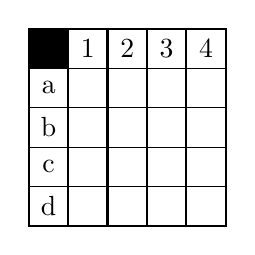
\begin{tikzpicture}[scale=0.5]
        \draw[thin,fill=black] (-1,0) rectangle (0,1);
\draw[ultra thin] (0,0) rectangle (1,1) (0.5,0.5) node {1};
\draw[ultra thin] (1,0) rectangle (2,1) (1.5,0.5) node {2};
\draw[ultra thin] (2,0) rectangle (3,1) (2.5,0.5) node {3};
\draw[ultra thin] (3,0) rectangle (4,1) (3.5,0.5) node {4};

            \draw[ultra thin] (-1,0) rectangle (0,-1) (-0.5,-0.5) node {a};
\draw [ultra thin,] (0,0) rectangle (1,-1);
\draw [ultra thin,] (1,0) rectangle (2,-1);
\draw [ultra thin,] (2,0) rectangle (3,-1);
\draw [ultra thin,] (3,0) rectangle (4,-1);

            \draw[ultra thin] (-1,-1) rectangle (0,-2) (-0.5,-1.5) node {b};
\draw [ultra thin,] (0,-1) rectangle (1,-2);
\draw [ultra thin,] (1,-1) rectangle (2,-2);
\draw [ultra thin,] (2,-1) rectangle (3,-2);
\draw [ultra thin,] (3,-1) rectangle (4,-2);

            \draw[ultra thin] (-1,-2) rectangle (0,-3) (-0.5,-2.5) node {c};
\draw [ultra thin,] (0,-2) rectangle (1,-3);
\draw [ultra thin,] (1,-2) rectangle (2,-3);
\draw [ultra thin,] (2,-2) rectangle (3,-3);
\draw [ultra thin,] (3,-2) rectangle (4,-3);

            \draw[ultra thin] (-1,-3) rectangle (0,-4) (-0.5,-3.5) node {d};
\draw [ultra thin,] (0,-3) rectangle (1,-4);
\draw [ultra thin,] (1,-3) rectangle (2,-4);
\draw [ultra thin,] (2,-3) rectangle (3,-4);
\draw [ultra thin,] (3,-3) rectangle (4,-4);
\draw [thick] (-1,1) rectangle (4,-4);
              %\draw [thick] (-1,0) -- (4,0);
              
\draw [thick] (0,1) -- (0,-4);
              
\draw [thick] (1,1) -- (1,-4);
              
\draw [thick] (2,1) -- (2,-4);
              
\draw [thick] (3,1) -- (3,-4);
              
\end{tikzpicture}\hfill\hfill\hfil
         % (introduction)

 % (introduction) % (sections) % shuffle sections
\section{Section 2}
\begin{enumerate}[resume] % shuffle sections % (questions) % shuffle questions
\item
\setcounter{answerNumber}{0} % (question) % pick a version
Question 4 % question % (answers)


\sloppy % shuffling answers
\stepcounter{answerNumber}\graysquared{\alph{answerNumber}}~~\mbox{ F}\qquad\linebreak[3]%
 % shuffling answers
\stepcounter{answerNumber}\graysquared{\alph{answerNumber}}~~\mbox{ V}\qquad\linebreak[3]%
 % (answers) % (question) % (section)
\end{enumerate} % shuffle sections
\section{Section 1}
\begin{enumerate}[resume] % shuffle sections % (questions) % shuffle questions
\item
\setcounter{answerNumber}{0} % (question) % pick a version
Question 3 % question (before l_answers)


\sloppy\stepcounter{answerNumber}\graysquared{\alph{answerNumber}}~~\mbox{N}\qquad\linebreak[3]%
\stepcounter{answerNumber}\graysquared{\alph{answerNumber}}~~\mbox{W}\qquad\linebreak[3]%
\stepcounter{answerNumber}\graysquared{\alph{answerNumber}}~~\mbox{E}\qquad\linebreak[3]%
\stepcounter{answerNumber}\graysquared{\alph{answerNumber}}~~\mbox{S}\qquad\linebreak[3]%

 % (question) % shuffle questions
\item
\setcounter{answerNumber}{0} % (question) % pick a version
 Question 1 bis % question % (answers)


\sloppy % shuffling answers
\stepcounter{answerNumber}\graysquared{\alph{answerNumber}}~~\mbox{ aa}\qquad\linebreak[3]%
 % shuffling answers
\stepcounter{answerNumber}\graysquared{\alph{answerNumber}}~~\mbox{ cc}\qquad\linebreak[3]%
 % shuffling answers
\stepcounter{answerNumber}\graysquared{\alph{answerNumber}}~~\mbox{ bb}\qquad\linebreak[3]%
 % (answers) % (answers) % shuffling answers
\stepcounter{answerNumber}\graysquared{\alph{answerNumber}}~~\mbox{ last answer}\qquad\linebreak[3]%
 % (answers) % (question)
\item
\setcounter{answerNumber}{0} % (question) % pick a version
Question 2 % question % (answers)


\sloppy % shuffling answers
\stepcounter{answerNumber}\graysquared{\alph{answerNumber}}~~\mbox{ 1}\qquad\linebreak[3]%
 % shuffling answers
\stepcounter{answerNumber}\graysquared{\alph{answerNumber}}~~\mbox{ 2}\qquad\linebreak[3]%
 % (answers) % (question) % (section)
\end{enumerate} % (sections)




\end{document}